\section{Tutorial Using Gravity and Finite Strain in Two Dimensions}
\label{sec:example:grav2d}

PyLith features discussed in this tutorial:
\begin{itemize}
\item Gravitational body forces (GravityField)
\item Initial stresses
\item Finite (or small) strain (ImplicitLgDeform)
\item Direct solver in simulations without a fault
\item Iterative solver with custom fault preconditioner for a fault
\item Generating a spatial database using h5py from state variables output
in HDF5 files
\item Cubit mesh generation
\item Quasi-static solution
\item Linear quadrilateral cells
\item Plane strain linearly elastic material
\item Plane strain Maxwell viscoelastic material
\item SimpleDB spatial database
\item ZeroDispDB spatial database
\item UniformDB spatial database
\end{itemize}
All of the files necessary to run the examples are contained under
the directory \filename{examples/2d/gravity. }The directory also contains
a \filename{README} file that describes the simulations and how to run
them.


\subsection{Overview}

This tutorial illustrates concepts related to using gravitational
body forces and finite (or small) strain. We focus on setting up initial
conditions consistent with gravitational body forces and using them
in a simulation of postseismic deformation with the small strain formulation.
We examine the differences between simulations with and without gravitational
body forces and the infinitesimal versus small strain formulation.

Steps 1-3 illustrate issues that arise when using gravitational body
forces and how to achieve realistic stress states. Steps 4-8 illustrate
the differences between infinitesimal and finite strain with and without
gravitational body forces for postseismic relaxation following an
earthquake with reverse slip.


\subsection{Problem Description}

The geometry of the problem is a 200km-wide by 100km-deep domain with
a flat ground surface. We use a 30km-thick elastic layer over a linear
Maxwell viscoelastic half-space to approximate the crust and mantle.
A reverse fault dipping 45 degrees cuts through the elastic layer
and extends into the top portion of the viscoelastic layer. Gravitational
body forces act in the vertical direction. We apply roller Dirichlet
boundary conditions to constrain the displacement normal to the boundary.

We discretize the domain using quadrilateral cells with a nominal
cell size of 2.0 km. We construct the mesh in CUBIT following the
same techniques used in the 2D subduction zone example, except that
this mesh is simpler. The main driver is in the journal file \filename{mesh.jou}.
It calls the journal file \filename{geometry.jou} to construct the geometry.
The mesh shown in Figure \vref{fig:examples:gravity:2d:mesh} The journal
files are documented and describe the various steps outlined below.
\begin{enumerate}
\item Create the geometry defining the domain.
\item Set the meshing scheme and cell size.
\item Generate the mesh.
\item Create blocks for materials and nodesets for boundary conditions.
\item Export the mesh.
\end{enumerate}

\begin{figure}
  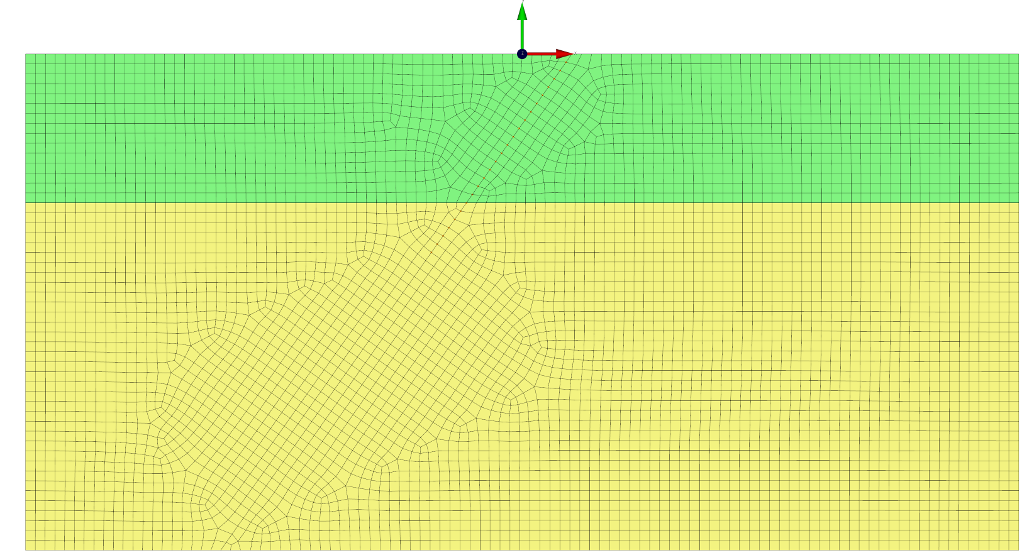
\includegraphics[width=4in]{examples/figs/grav2d_mesh}
  \caption{Mesh used for 2d gravity simulations with a 30 km thick elastic crust
    over a 70 km thick linear Maxwell viscoelastic layer.}
  \label{fig:examples:gravity:2d:mesh}
\end{figure}


\subsection{Additional Common Information}

As in the examples discussed in previous sections of these tutorials,
we place parameters common to all of the simulations in the \filename{pylithapp.cfg}
file so that we do not have to duplicate them in each simulation parameter
file. In some cases we do override the values of parameters in simulation
specific parameter files. The settings contained in \filename{pylithapp.cfg}
for this problem consist of:
\begin{inventory}
  \facilityitem{pylithapp.journal.info}{Settings that control the verbosity of
    the output written to stdout for the different components.}
  \facilityitem{pylithapp.mesh\_generator}{Settings that control mesh importing,
    such as the importer type, the filename, and the spatial dimension
    of the mesh.}
  \facilityitem{pylithapp.problem}{Settings that control the problem, such as
    the total time, time-step size, and spatial dimension. Note that we
    turn off the elastic prestep here, since it is only used in the first
    simulation. We also turn on gravity for the problem. The \texttt{total\_time}
    of \texttt{2000.0{*}year }is used for most of the simulations.}
  \facilityitem{pylithapp.problem.materials}{Settings that control the material
    type, specify which material IDs are to be associated with a particular
    material type, and give the name of the spatial database containing
    the physical properties for the material. The quadrature information
    is also given.}
  \facilityitem{pylithapp.problem.bc}{We apply Dirichlet roller boundary conditions
    (pin displacement perpendicular to the boundary) on the lateral sides
    and bottom of the domain.}
  \facilityitem{pylithapp.problem.formulation.output}{Settings related to output
    of the solution over the domain and subdomain. We specify both displacements
    and velocities for the output.}
  \facilityitem{pylithapp.petsc}{PETSc settings to use for the problem, such as
    the preconditioner type.}
\end{inventory}
Since we do not desire an initial elastic solution prior to beginning
our time stepping for the simulations, we turn off the elastic prestep:
\begin{cfg}
<h>[pylithapp.timedependent]</h>
<p>elastic_prestep</p> = False
\end{cfg}
For two-dimensional problems involving gravity, we also need to change
the default \property{gravity\_dir}:
\begin{cfg}
<h>[pylithapp.timedependent]</h>
<f>gravity_field</f> = spatialdata.spatialdb.GravityField
<p>gravity_field.gravity_dir</p> = [0.0, -1.0, 0.0]
\end{cfg}

\subsection{Step 1: Gravitational Body Forces and Infinitesimal Strain}

This simulation applies gravitational body forces to a domain without
any initial conditions, so the gravitational body forces cause the
domain to compress in the vertical direction. The shear stresses in
the mantle relax, so that the solution in the mantle trends towards
$\sigma_{xx}=\sigma_{yy}$. The crust is elastic and compressible, so
$\sigma_{xx}\neq\sigma_{\mathit{yy}}$. In the earth's crust we
generally observe $\sigma_{\mathit{xx}}\approx\sigma_{\mathit{yy}}$,
so this simulation does not yield a stress state consistent with that
observed in nature. The file \filename{gravity\_infstrain.cfg}
contains the simulation specific parameter settings that augment those
in \filename{pylithapp.cfg}.  In addition to the filenames for the
HDF5 ouput we also set the filename for the progress monitor. You can
look at this file during the simulation to monitor the progress and
get an estimate of when the simulation will finish.

We run the simulation using:
\begin{shell}
$$ pylith gravity_infstrain.cfg
\end{shell}
The simulation produces HDF5 (and corresponding XDMF) files with the
output of the displacements on the ground surface and the entire
domain, and the state variables for the crust and mantle. Note that
the output files contain both cauchy\_stress and stress fields. For
problems using the infinitesimal strain formulation, these are
identical. For the small strain formulation, the stress field
corresponds to the second Piola-Kirchoff stress tensor, which does not
have the physical meaning associated with the Cauchy stress. Loading
the axial stress fields for the crust and mantle into ParaView via the
XDMF files (\filename{output/gravity\_infstrain-crust.xmf} and
\filename{output/gravity\_infstrain-mantle.xmf}) illustrates how the
axial stresses are not equal. We would like gravitational body forces
to yield nearly axial stresses consistent with the overburden pressure
observed in nature.


\subsection{Step 2: Gravitational Body Forces, Infinitesimal Strain, and Initial Stresses}

This simulation uses depth-dependent initial stresses that satisfy the
governing equations. As a result, there is zero deformation. In
practice, there would be no need to run such a simulation, because the
initial stresses give us the stress state produced in the simulation.
In Steps 3-7, we use these initial stresses as initial conditions for
postseismic deformation simulations. Because we reuse the initial
stress parameter settings in multiple simulations, we place them in
their own parameter file, \filename{gravity\_initstress.cfg}. As in
Step 1, the simulation specific parameter file contains the filenames
for the output.

We run the simulation using:
\begin{shell}
$$ pylith gravity_initstress.cfg gravity_isostatic.cfg
\end{shell}

\subsection{Step 3: Infinitesimal Strain Simulation with Initial Stresses and
a Local Density Variation}

This simulation adds a local density variation in the elastic layer
to the problem considered in Step 2. Near the origin, the density
is reduced in a semi-circular region with a radius of 5.0 km, roughly
approximating a sedimentary basin. In this example, we focus on the
workflow and use a coarse mesh so we are not concerned with the fact
that our mesh with a discretization size of 2.0 km does a poor job
of resolving this density variation; in a real research problem we
would use a finer mesh in the low density region. Figure \vref{fig:examples:gravity:2d:vardensity:density}shows
the spatial variation in density, including the contrast in density
between the mantle and crust and the circular low density region around
the origin.

\begin{figure}
  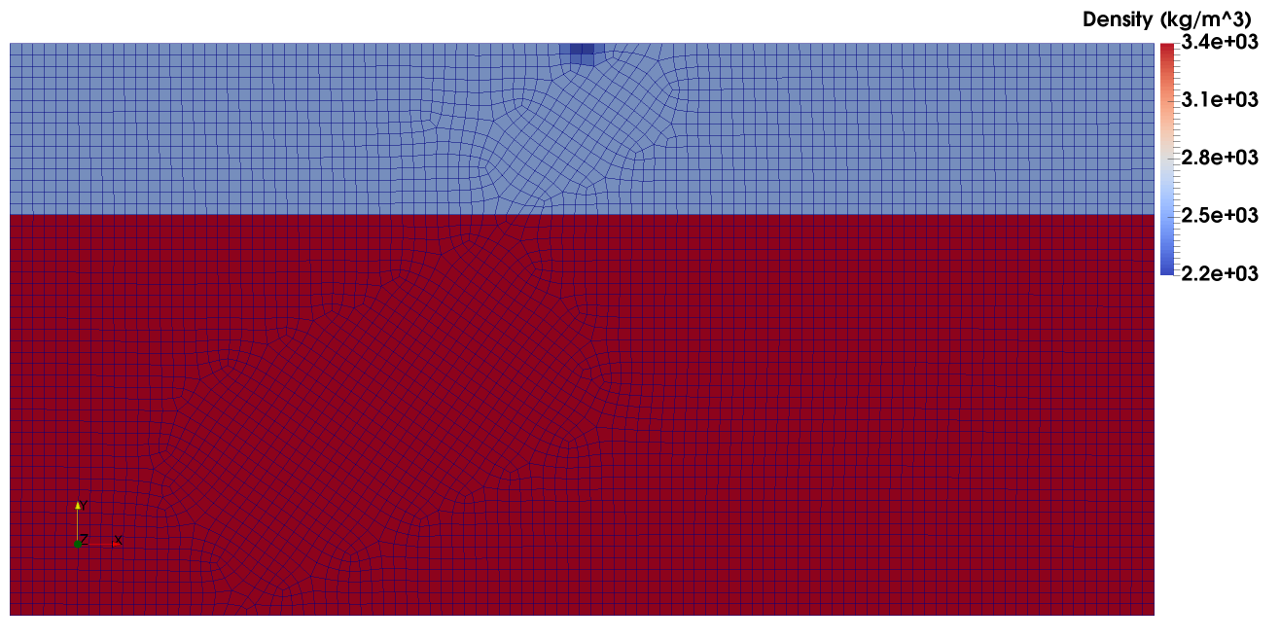
\includegraphics[width=4in]{examples/figs/grav2d_vardensity-density}
  \caption{Spatial variation in density in the finite element mesh. The mantle
    has a uniform density of 3400 kg/m$^{3}$ and the crust has a uniform
    density of 2500 kg/m$^{3}$ except near the origin where we impose
    a low density semi-circular region.}
  \label{fig:examples:gravity:2d:vardensity:density}
\end{figure}

We use the same initial stress state as for the previous two examples.
The initial stress state is a close approximation to the equilibrium
state, so there is little deformation. The mantle relaxes
corresponding to the viscous strains and shear stresses approaching
zero; shear stress associated with the lateral density variation
becomes confined to the crust. In the region with the lower density,
the initial stresses do not satisfy the governing equation and the
solution slowly evolves towards a steady state. This slow asymptotic
evolution presents some difficulties with using the output of this
simulation (which has not reached the equilibrium state) as a starting
point in other simulations, as we will see in Step 8. Nevertheless,
this simulation serves as an example of how to use initial stresses
from vertically layered material properties in computing an
equilibrium or steady state stress state associated with gravitational
body forces and lateral density variations or topography.

We run the simulation using:
\begin{shell}
$$ pylith gravity_initstress.cfg gravity_vardensity.cfg
\end{shell}
Figure \vref{fig:examples:gravity:2d:vardensity:stress} shows the
shear stress field at the end of the simulation.

\begin{figure}
  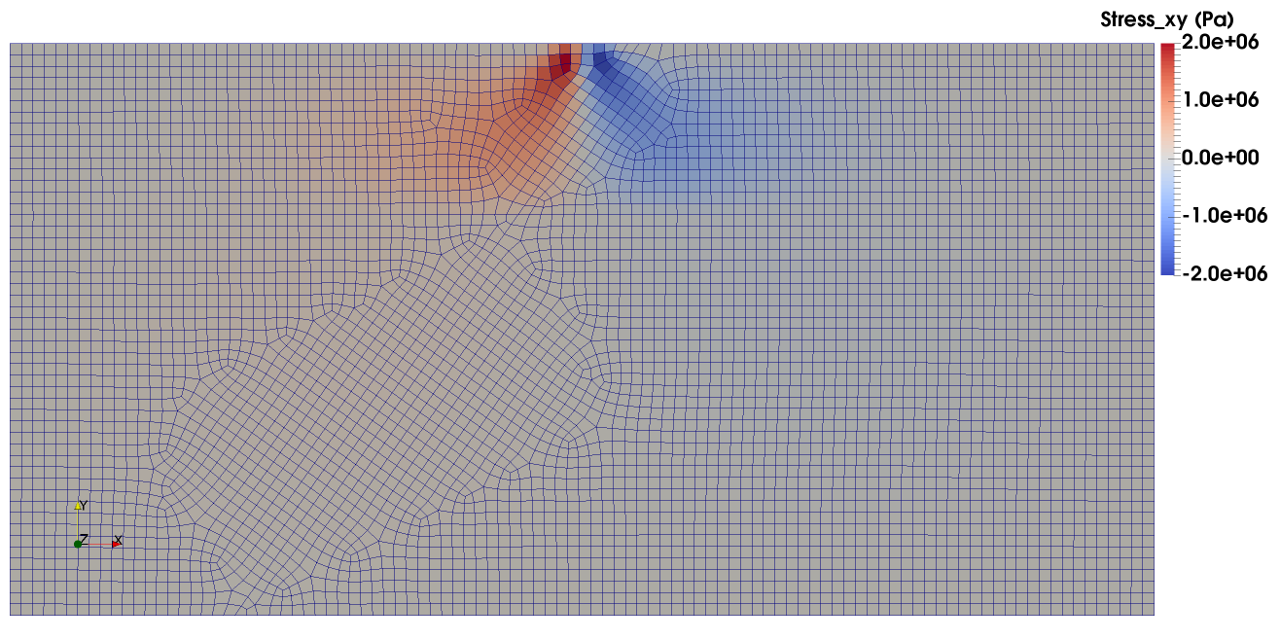
\includegraphics[width=4in]{examples/figs/grav2d_vardensity-shearstress}
  \caption{Shear stress in the crust (linearly elastic) and mantle
    (linear Maxwell viscoelastic) associated gravitational body forces
    and a low density region forces.}
  \label{fig:examples:gravity:2d:vardensity:stress}
\end{figure}


\subsection{Step 4: Postseismic Relaxation with Infinitesimal Strain}

We impose slip on the reverse fault within the elastic layer and
compute the postseismic deformation associated with relaxation in the
mantle.  We do not include gravitational body forces. The earthquake
slip is 2.0 m above a depth of 15 km and tapers linearly to zero at a
depth of 20 km. We impose the earthquake at time 0.0 years, but use a
start time of -100 years so that any pre-earthquake deformation trends
are clear. We use one parameter file (\filename{nogravity.cfg}) to
turn off gravity (by setting the gravitional acceleration to zero) and
another parameter file (\filename{postseismic.cfg}) for the earthquake
related parameters. Note that we change the preconditioner to the
algebraic multigrid preconditioner for the elastic block and the
custom fault preconditioner for the Lagrange multipliers.

We run the simulation using:
\begin{shell}
$$ pylith postseismic.cfg nogravity.cfg postseismic_infstrain_nograv.cfg
\end{shell}
Figure \vref{fig:examples:gravity:2d:postseismc:infstrain:disp} shows
the vertical displacement field at the end of the simulation.

\begin{figure}
  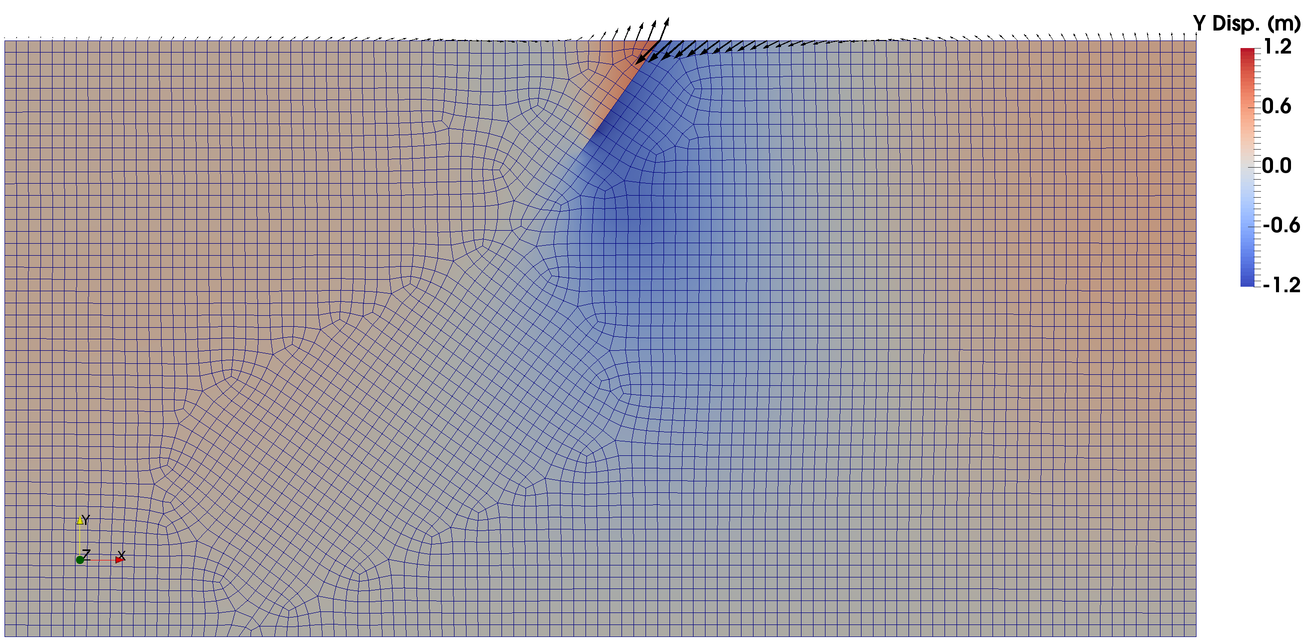
\includegraphics[width=4in]{examples/figs/grav2d_postseismic_infstrain_nograv-disp}
  \caption{Vertical displacement at the end of the postseismic deformation simulation
    (t=4000 years).}
  \label{fig:examples:gravity:2d:postseismc:infstrain:disp}
\end{figure}


\subsection{Step 5: Postseismic Relaxation with Finite Strain}

This simulation is the same as Step 4, but we use the finite strain
formulation.:
\begin{cfg}
<h>[pylithapp.timedependent]</h>
<f>formulation</f> = pylith.problems.ImplicitLgDeform
\end{cfg}
When we use the finite strain formulation, the solver is automatically
switched to the nonlinear solver. We run the simulation using:
\begin{shell}
$$ pylith postseismic.cfg nogravity.cfg postseismic_finstrain_nograv.cfg
\end{shell}
The results are nearly identical to those with infinitesimal strain.


\subsection{Step 6: Postseismic Relaxation with Infinitesimal Strain and Gravitational Body Forces}

This simulation is the same as Step 4, but we include gravitational
body forces. We use initial stresses that satisfy the governing
equations, so our initial conditions are axial stresses equal to the
overburden pressure.

We run the simulation using:
\begin{shell}
$$ pylith postseismic.cfg postseismic_infstrain.cfg
\end{shell}
With the infinitesimal strain formulation and linearly material behavior,
the initial stress state of equal axial stresses does not alter the
response. We obtain a displacement field and shear stresses identical
to that in Step 4. The axial stresses are the superposition of the
initial stresses and those from the postseismic deformation.


\subsection{Step 7: Postseismic Relaxation with Finite Strain and Gravitational Body Forces}

This simulation is the same as Step 5, but we include gravitational
body forces; this is also the same as Step 6, but with finite strain.

We run the simulation using:
\begin{shell}
$$ pylith postseismic.cfg postseismic\_finstrain.cfg
\end{shell}
The finite strain formulation accounts for the redistribution of
gravitational body forces as the domain deforms during the postseismic
response.  As a result, the displacement field differs from that in
Steps 4-6.  To see this difference, we have created a ParaView state
file to view the ground surface deformation from the output of Steps
4-7. After running all four simulations, open ParaView and load the
state file \filename{postseismic.pvsm}. If you start ParaView from the
\filename{examples/2d/gravity} directory
(\filename{PATH\_TO\_PARAVIEW/bin/paraview},
\texttt{File$\rightarrow$Load State$\rightarrow$postseismic.pvsm}),
you should not need to update the locations of the filenames. If you
start ParaView from a dock or other directory, you will need to set
the relative or absolute paths to the output files. Figure
\vref{fig:examples:gravity:2d:postseismic:groundsurf} shows the ground
deformation 2550 years after the earthquake using the state file.

\begin{figure}
  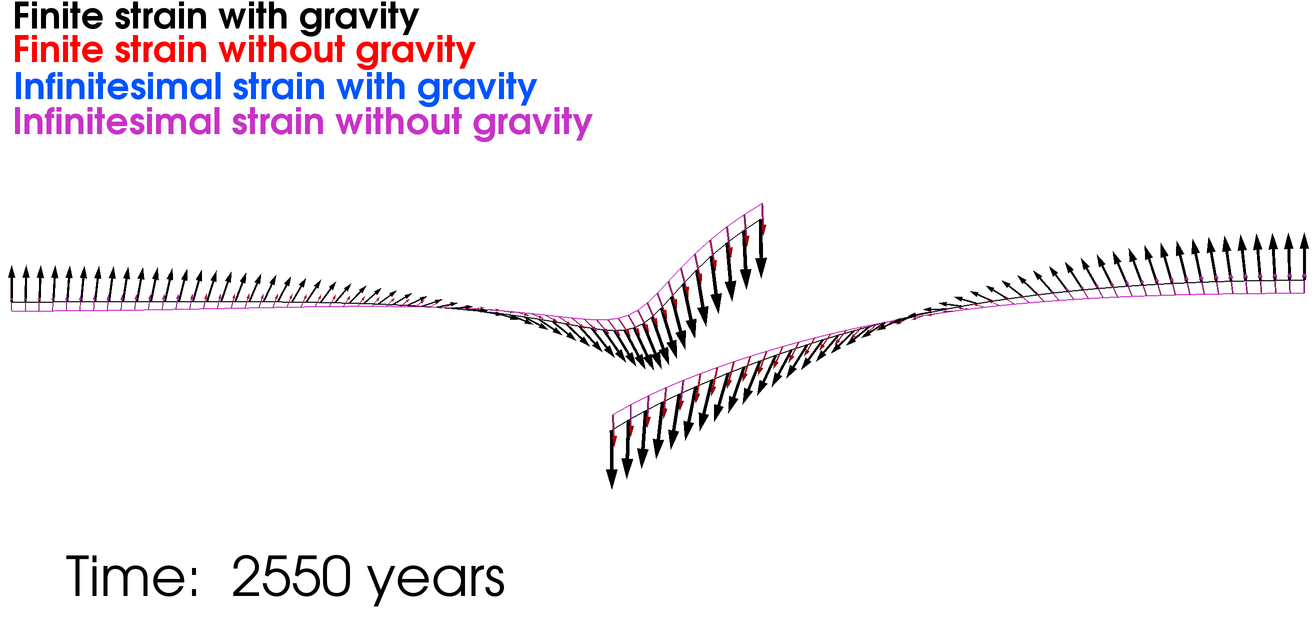
\includegraphics[width=4in]{examples/figs/grav2d_postseismic_dispcmp}
  \caption{Displacement field on the ground surface after 2550 years
    of postseismic deformation in Step 4 (Infinitesimal strain without
    gravity), Step 5 (Finite strain without gravity), Step 6
    (Infinitesimal strain with gravity), and 7 (Finite strain with
    gravity). The displacement fields for Steps 4-6 are essentially
    identical.}
  \label{fig:examples:gravity:2d:postseismic:groundsurf}
\end{figure}


\subsection{Step 8: Postseismic Relaxation with Finite Strain, Gravitational
Body Forces, and Variable Density}

We use the output of Step 3 to create realistic initial stresses for
this simulation of postseismic deformation with variable density.
In Step 3 we average the stresses over the quadrature points within
a cell using CellFilterAvg. For initial stresses consistent with the
state of the simulation at the end of Step 3, we want the stresses
at each of the quadrature points. Note that Step 3 uses the infintesimal
strain formulation and for Step 8 we will use a finite strain formulation;
any inconsistencies in using the output from a simulation with one
strain formulation as the input in a simulation for another strain
formulation are very small given that we start Step 8 from an undeformed
state so that the Cauchy stresses are very close to the second Pioloa-Kirchoff
stresses. Our first step is to modify the \filename{pylithapp.cfg} file
by commenting out the lines with the CellFilterAvg settings:
\begin{cfg}
# If rerunning Step 3 to get initial conditions for Step 8, comment out the next line as shown.
#cell_filter = pylith.meshio.CellFilterAvg
\end{cfg}
for both the crust and mantle. Next we rerun Step 3 using
\begin{shell}
$$ pylith gravity_initstress.cfg gravity_vardensity.cfg
\end{shell}
This will change how the values appear in ParaView output. Because
the output data fields contain the values at multiple points within
a cell, PyLith does not label them as tensor components; instead,
it simply numbers the values 0..N. For the stress tensor components,
values 0, 1, and 2 are the $\sigma_{\mathit{xx}}$, $\sigma_{\mathit{yy}}$,
and $\sigma_{\mathit{xy}}$ values at the first quadrature point;
values 3, 4, and 5 correspond to the values at the second quadrature
point, etc. We use the Python script \filename{generate\_statedb.py}
to generate the spatial databases with the initial stresses from the
output of Step 3:
\begin{shell}
$$ ./generate_statedb.py
\end{shell}
After generating the initial state variables, we uncomment the \texttt{cell\_filter}
lines in \filename{pylithapp.cfg} to allow easier visualization of Step
8 results. Finally, we run the simulation of the postseismic deformation
using
\begin{shell}
$$ pylith postseismic.cfg gravity_initstress.cfg postseismic_vardensity.cfg
\end{shell}
In the 100 years before the earthquake, it is clear that there is
some ongoing deformation associated with the relaxation of the mantle.
Immediately following the earthquake the postseismic deformation signal
is stronger at most locations, but as it decays the ongoing deformation
associated with the gravitational body forces and variable density
become evident again. This ongoing deformation is most obvious in
the displacement and velocity fields. The postseismic deformation
is much more dominant for the stress field. This contamination by
the initial conditions can be avoided with initial stress conditions
at equilibrium as we did in Step 7. However, this is much more difficult
to obtain for complex lateral variations in density or topography.
Figure \vref{fig:examples:gravity:2d:postseismic:vardensity:shearstress}
shows the ground deformation at time 2000 years into the simulation
using the state file. 

\begin{figure}
  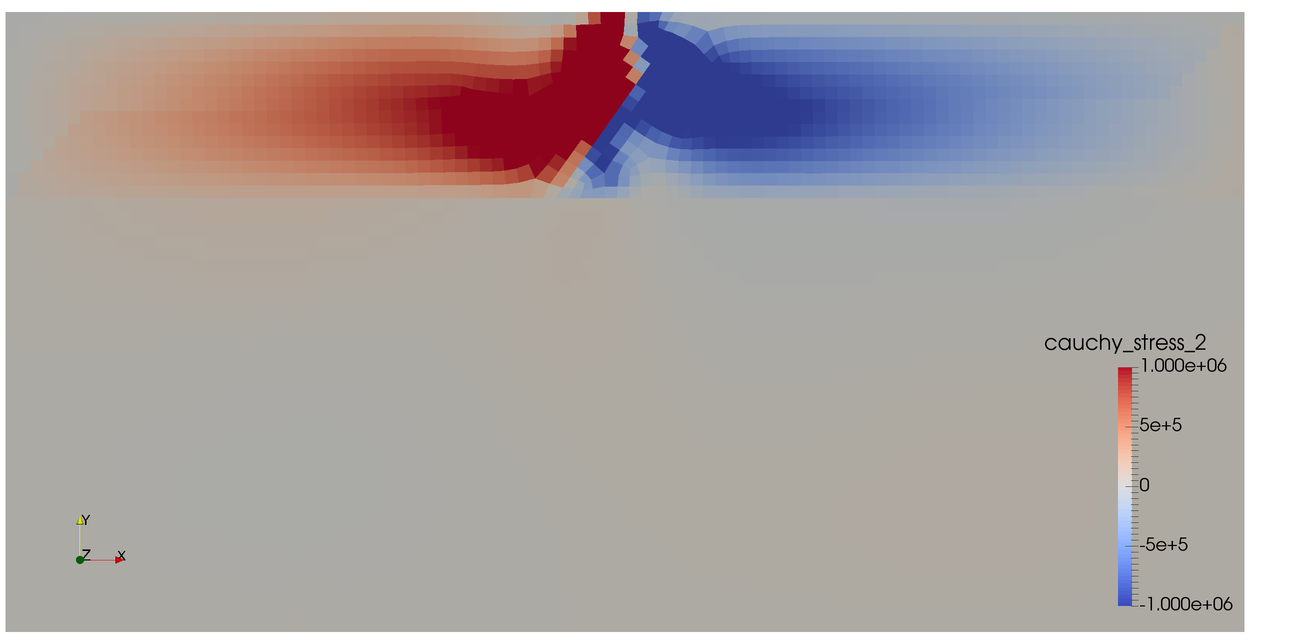
\includegraphics[width=4in]{examples/figs/grav2d_postseismic_vardensity-shearstress}
  \caption{Cauchy shear stress at the end of the simulation of postseismic deformation
    with variable density in the crust. We saturate the color scale at
    $\pm$1 MPa to show the evidence of viscoelastic relaxation (near
    zero shear stress) in the mantle.}
  \label{fig:examples:gravity:2d:postseismic:vardensity:shearstress}
\end{figure}

\subsection{Exercises}

The \filename{README} file in \filename{examples/2d/gravity} includes
some suggetions of additional simulations to run to further explore
some of the issues discussed in this suite of examples.

% End of file
